% !TeX spellcheck = en_US
\newpage
\section{Microarchitecture}
This section describes level no. 1 from the 6 level model that we saw in \ref{img:levels}.
\subsection{Architecture of a microprocessor}
The internal architecture of a simple microprocessor is designed as follows:
\begin{center}
	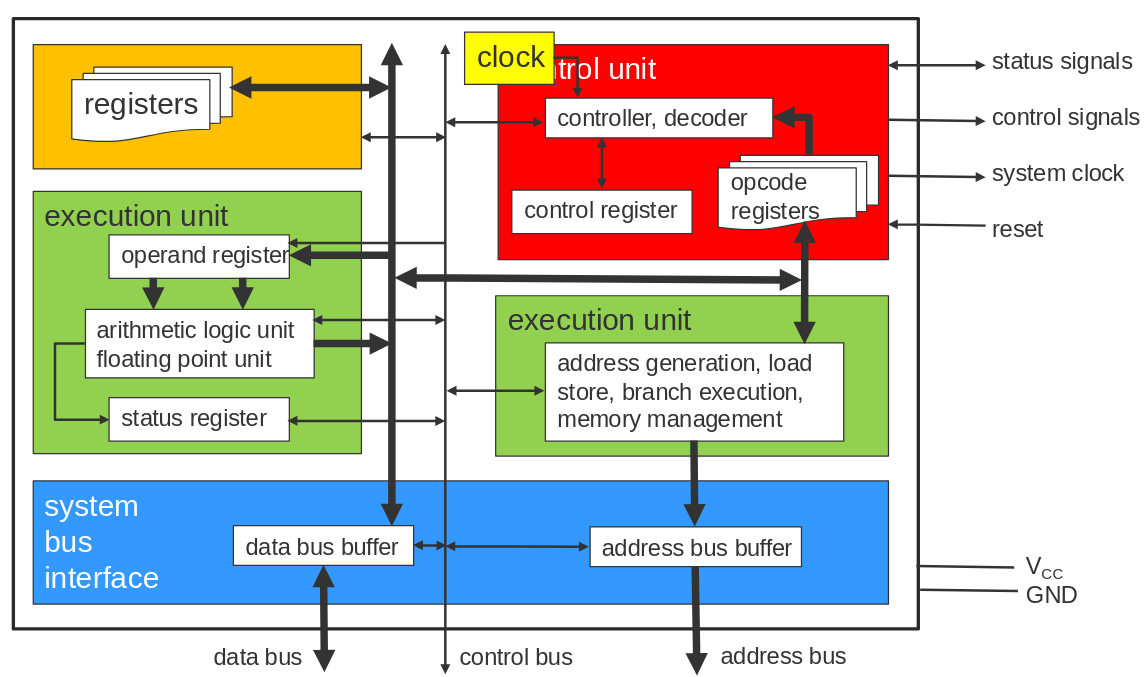
\includegraphics[scale=0.35]{microarchitecture}
\end{center}

\subsubsection{Control unit}

\begin{wrapfigure}[4]{r}{6cm}
	\vspace{-1.1cm}
	\begin{center}
		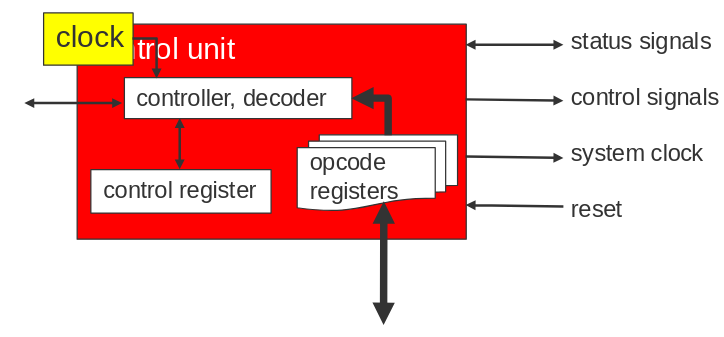
\includegraphics[width=6cm]{controlunit}
	\end{center}
\end{wrapfigure}

The control unit is the part that \textbf{controls} all the other components.
\paragraph{Clock} Generates the system clock for distribution to all components.

\paragraph{Decoder} 
It generates all control signals for the components and uses status signals and opcode as an input. Often \textbf{micro-programmable}.

\begin{definition}[Micro programmable]
	The processor stores a \textbf{microprogram} for each instruction that can be modified only by the manufacturer. Single bits of a \textbf{micro instruction} represents \textbf{micro operations}, thus a setting of the control signals for the components.\\
	Pure \textbf{RISC} processors typically use a fixed sequential circuit instead.
\end{definition}

\noindent The \textbf{phases of execution} of an instruction is composed of:
\begin{enumerate}
	\item \textbf{Fetch}: load the next instruction into the opcode register
	\item \textbf{Decode}: get the start address of the microprogram representing the instruction
	\item \textbf{Execute}: the microprogram controls the instruction execution by sending the appropriate signals to the other components and evaluating the returned signals
\end{enumerate}

\paragraph{Opcode register}
It contains the portion of the \textbf{instruction} that specifies the currently executed operation to be performed and eventual \textbf{opcodes}. It has \textbf{several registers} because:
\begin{itemize}
	\item Different instructions may have \textbf{different sizes}
	\item Opcode \textbf{prefetching} may speed up program execution: while decoding the current instruction the following one may be prefetched
\end{itemize}

\paragraph{Control register}
It stores the current status of the control unit. The meaning of the different bits depend on the specific processor. Some examples:
\begin{itemize}
	\item \textit{Interrupts} enable: determines if the processor reacts to interrupts
	\item \textit{VM extension} enable: enable HW assisted virtualization on x86 CPUs
	\item \textit{User mode instruction prevention}: if set, certain instructions cannot be executed in user level
\end{itemize}

\subsubsection{Execution unit}
\begin{wrapfigure}[8]{r}{5cm}
	\vspace{-0.5cm}
	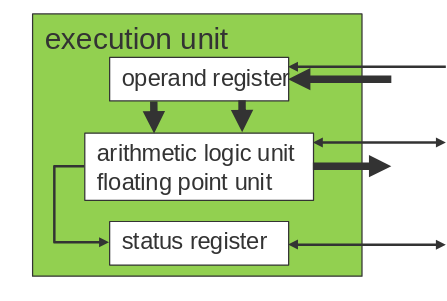
\includegraphics[width=5cm]{execunit1}
\end{wrapfigure}
The execution unit executes all \textbf{logic} and \textbf{arithmetic operations} controlled by the control unit (e.g. int and float arithmetic, logic operations, address operations).

\paragraph{Communication with control unit}
Single bits of a micro instruction directly control the ALU operation and its operands.
\begin{example}
	Example of micro instruction that sets $S_3$, $S_4$ and $S_5$:
	\begin{center}
		\begin{table}[!h]
			\centering
			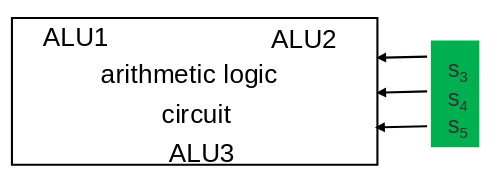
\includegraphics[scale=0.25]{execexample}
			\begin{tabular}{|c|c|c|c|}
				\hline
				$S_3$ & $S_4$ & $S_5$ & $\text{ALU}_3$ \\
				\hline
				0 & 0 & 0 & $\text{ALU}_1 + \text{ALU}_2 + C_{in}$ \\
				\hline
				0 & 0 &1 & $\text{ALU}_1 - \text{ALU}_2 - (\neg C_{in})$ \\
				\hline
				0 & 1 & 0 & $\text{ALU}_2 - \text{ALU}_1 - (\neg C_{in})$ \\
				\hline
				0 & 1 & 1 & $\text{ALU}_1 \lor \text{ALU}_2$ \\
				\hline
				1 & 0 &0 & $\text{ALU}_1 \land \text{ALU}_2$ \\
				\hline
				1 & 0 & 1 & $(\neg \text{ALU}_1) \land \text{ALU}_2$ \\
				\hline
				1 & 1 & 0 & $\text{ALU}_1 \oplus \text{ALU}_2$ \\
				\hline
				1 & 1 &1 & $\text{ALU}_1 \leftrightarrow \text{ALU}_2$ \\
				\hline
			\end{tabular}
		\end{table}
	\end{center}
\end{example}

\paragraph{Status register}
Informs the control unit about the state of the processor after an operation via single bits. Common \textbf{flags} (the bits) are:
\begin{itemize}
	\item \textbf{Auxiliary Carry} (AF): indicates a carry between the \textit{nibbles} (4bit halves of a byte). It's used for \textbf{binary coded digit} arithmetic. \footnote{Also called \textit{half-carry flag}, \textit{digit carry}, \textit{decimal adjust flag}.} 
	\item \textbf{Carry Flag} (CF): indicates a carry produced by the MSBs. Allows for additions and subtractions between \textbf{numbers larger} that a single word through sequential operations that take the carry into account.
	\item \textbf{Zero Flag} (ZF): if the result of an operation was zero. Used for \textbf{conditional branches}.
	\item \textbf{Even Flag} (EF): if the result is \textbf{even} or \textbf{odd} based on the LSB
	\item \textbf{Sign Flag} (SF): if the result is negative (MSB is 1) in two complements. Used for \textbf{conditional branches}.
	\item \textbf{Parity Flag} (PF): if the number of set bits is even or odd. Used for \textbf{error detection}.
	\item \textbf{Overflow Flag} (OF): if the result of an operation is too large to be represented 
\end{itemize}

\paragraph{Program Status Word}
Status register combined with control register determine the current \textbf{state} of a processor. If we combine that with the \textbf{program counter} we get the state of a processor at a certain instruction of a program. It gets:
\begin{itemize}
	\item \textbf{Pushed} to stack before context switch
	\item \textbf{Pulled} from stack to continue execution of an interrupted program
\end{itemize}

\paragraph{Address generation unit}
\begin{wrapfigure}[3]{r}{3.3cm}
	\vspace{-0.5cm}
	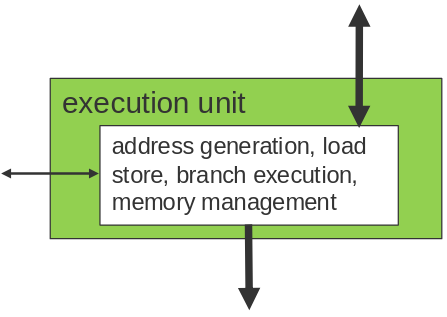
\includegraphics[width=3.3cm]{execunit2}
\end{wrapfigure}
Calculates the address based on control signals from the control unit and possible additional content of the registers.

\subsubsection{Registers}
\begin{wrapfigure}[10]{r}{8cm}
	\vspace{-1cm}
	\begin{center}
		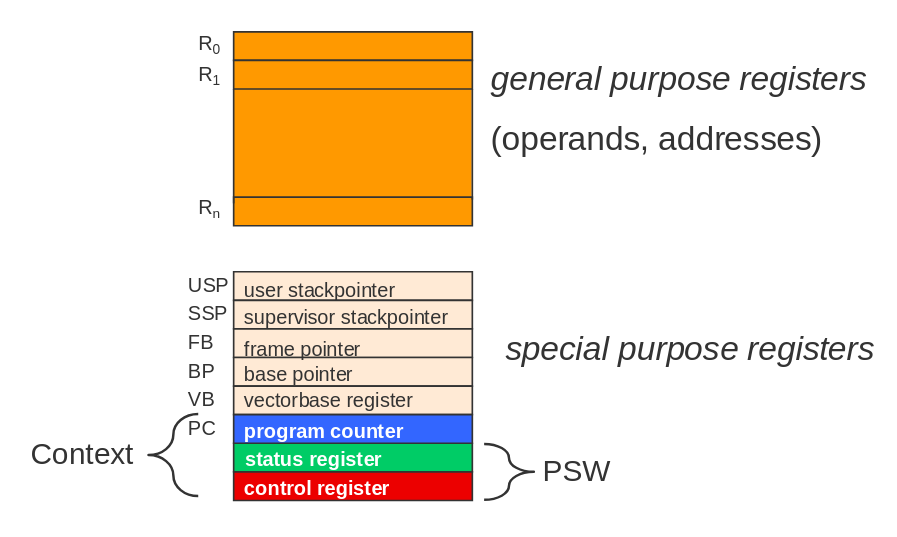
\includegraphics[width=8cm]{registerfile}
	\end{center}
\end{wrapfigure}
They extend the registers of the execution unit, containing frequently used operands. It's a very \textbf{fast} memory with a low access time ($<1\text{ms}$).\\
The \textbf{selection} of single registers happens through dedicated \textbf{control lines} without any address decoding. It can also offer other functions:
\begin{itemize}
	\item \textbf{Increment} and \textbf{decrement}
	\item \textbf{Shift}
	\item Set to \textbf{zero}
\end{itemize}
There are several independent I/O ports, allowing \textbf{simultaneous} writing and reading of different registers. In modern processors up to 4 writes and 8 reads in one clock cycle.

\paragraph{Base pointer}
The base pointer special register contains the start address of a memory region (e.g. an array). The \textbf{index} represents the offset relative to the base pointer. The sum of the two gives the absolute address of an element.

\begin{center}
	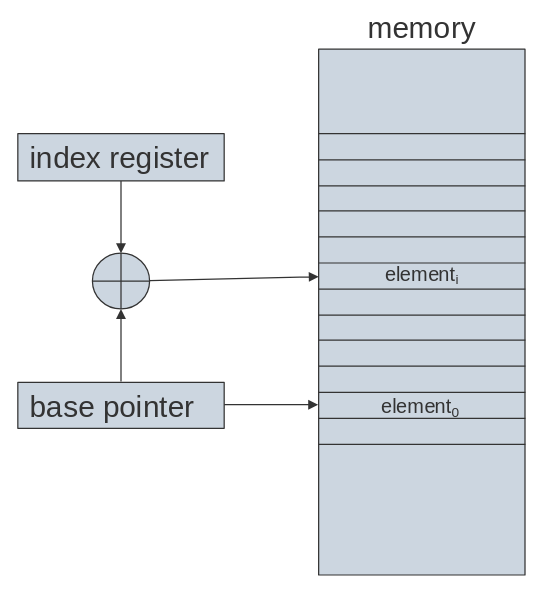
\includegraphics[scale=0.3]{basereg}
\end{center}

\paragraph{Index register}
\noindent The \textbf{index register} has special functions to save time from the ALU:
\begin{itemize}
	\item \textbf{Post-increment}: automatic increment of the register by $n$ after addressing the memory
	\item \textbf{Pre-decrement}: automatic decrement of the register by $n$ before addressing the memory
	\item \textbf{Auto-increment/decrement}
	\item \textbf{Autoscaling} by a factor $n$, used to access memory in bytes or words
\end{itemize}

\paragraph{Stack pointer}
Part of the main memory organized with \textbf{LIFO} principle. It stores the \textbf{PSW} during the subroutine calls/interrupts, allows the passing of the \textbf{parameters} and stores \textbf{temporary results}. Processors usually have different types (e.g. user, system, data).\\
The \textbf{stack pointer} contains the address of the newest data on the stack.\\
Two operations are allowed:
\begin{itemize}
	\item \textbf{PUSH}: transfer the value of a register on top of the stack
	\item \textbf{POP}: load a register with the value on top of the stack and remove it
\end{itemize}

\subsubsection{System Bus Interface}
The Bus Interface Unit is the connection of the microprocessor to all the other components of the computer. The main purposes are:
\begin{itemize}
	\item \textbf{Buffering} of \textit{addresses} and \textit{data} (operand and instructions)
	\item \textbf{Adaptation} of \textit{clock cycle}, \textit{bus width} and \textit{voltages}
	\item \textbf{Tristate}: detaches the processor from the external bus
\end{itemize}
\begin{center}
	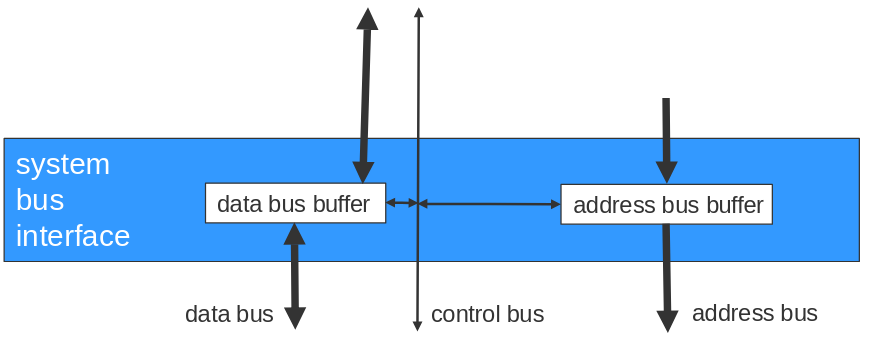
\includegraphics[scale=0.4]{bus}
\end{center}

\subsection{Pipelining}
The performance of a computer can be improved either by improving the \textbf{hardware} using new technologies and materials (expensive and with limitations) or by increasing the \textbf{parallelism} (more transistors, wider bus, replicated function units).

\subsubsection{Structural enhancements}
The classification of computer architectures, according to Flynn, is composed of four types.
\paragraph{SISD} Single Instruction Single Data consists in one single stream of instructions that operate on the data (classic Von Neumann).

\paragraph{SIMD} Single Instruction Multiple Data is where all processors perform the same instruction on different data (array processor). E.g. image processing, where each processor handle one part of the image.

\paragraph{MIMD} Multiple Instruction Multiple Data where all processors perform different instructions on different data. The one it's mostly used today.

\paragraph{MISD} Multiple Instruction Single Data where several instructions operate on a single data. Not very common but could be use e.g. for fault tolerance (and then compare the results).

\begin{figure}[!h]
	\hfill
	\subfigure[SISD]{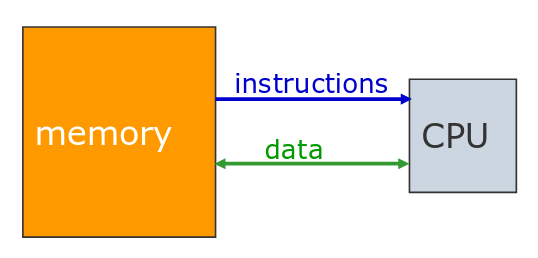
\includegraphics[scale=0.2]{sisd}}
	\hfill
	\subfigure[SIMD]{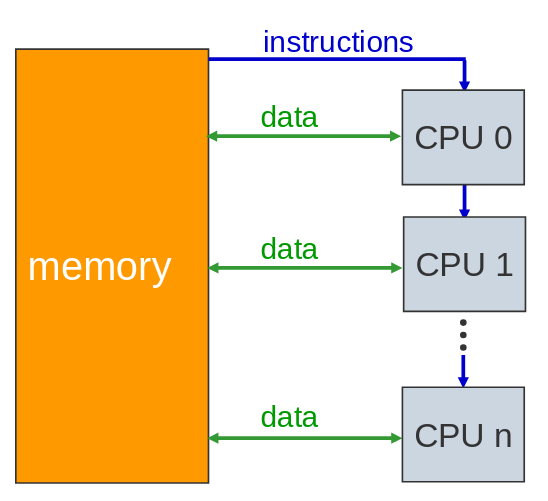
\includegraphics[scale=0.2]{simd}}
	\hfill
	\subfigure[MIMD]{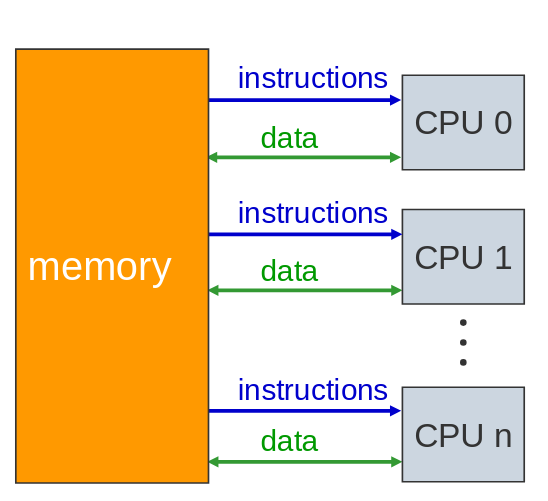
\includegraphics[scale=0.2]{mimd}}
	\hfill
\end{figure}

\subsubsection{Pipeline processing}
Pipelining is the \textbf{subdivision} of an operation into several phases or sub operations and their \textbf{synchronous execution} in different functional unit (each one responsible for its own).\\
Each stage is a pipeline \textbf{stage} or \textbf{segment}. The whole pipeline is clocked in a way that each cycle instruction can be shifted one step further through it.\\
Ideally we have a $\mathbf{k}$ \textbf{stage pipeline} with $k$ cycles and $k$ stages, allowing $k$ instructions to be executed at the same time and needing $k$ cycles to complete.

\begin{definition}[Latency]
	Duration of the complete processing of an instruction. The time an instruction needs to go through	all $k$ stages of the pipeline.
\end{definition}

\begin{definition}[Throughput]
	Number of instructions leaving the pipeline per clock cycle. It should be close to $1$ for a \textbf{scalar} processor and may be $> 1$ for \textbf{superscalar} processors.
\end{definition}

\paragraph{Speedup}
A \textbf{standard} processor without pipeline, considering $n$ instructions and $k$ stages, needs:
\begin{equation}
	n \cdot k \text{ cycles}
\end{equation}
A \textbf{pipelined} processor needs, assuming $k$ cycles latency and throughput $=1$, needs:
\begin{equation}
	k + (n-1) \text{ cycles}
\end{equation}
Assuming an infinite number of instructions the \textbf{speed up} of a processor with a $k$ staged pipeline is:
\begin{equation}
	\lim_{n \to \infty} \frac{n \cdot k}{k+n-1} = \lim_{n \to \infty} \frac{k}{\frac{k}{n}+1-\frac{1}{n}} = \frac{k}{0+1-0} = k
\end{equation}

\paragraph{Five stage pipeline}
It consists in these five stages:
\begin{enumerate}
	\item \textbf{Instruction Fetch} (IF): load the instruction from memory or cache into the opcode register and increment the program counter
	\item \textbf{Instruction Decode} (ID): generate internal signals based on the opcode or jump to the appropriate microprogram
	\item \textbf{Operand Fetch} (OF): load the operands from the registers into the operand registers of the ALU and calculate the effective address for load/store or branch instructions
	\item \textbf{Execution} (EXE)
	\item \textbf{Write Back} (WB): write the result into a register or memory if needed. Load/store instructions put the address on the address bus and transfer the data to the memory
\end{enumerate}
\begin{center}
	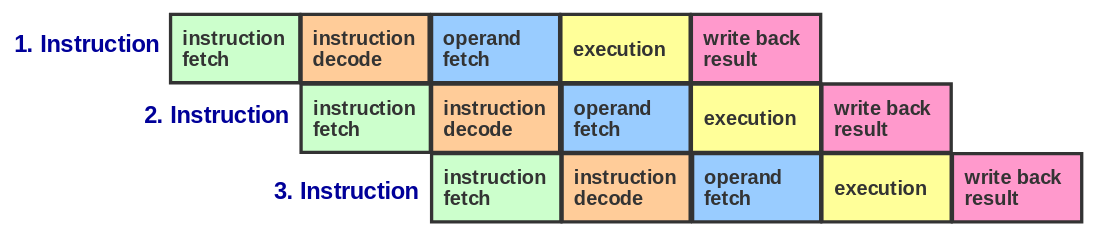
\includegraphics[scale=0.3]{pipeline}
\end{center}

\paragraph{Two instruction}
If we assume that:
\begin{itemize}
	\item Instruction Fetch requires half the time of all other stages
	\item We can have arbitrary many other functional units
\end{itemize}
then we can have an improved pipeline that works in parallel:
\begin{center}
	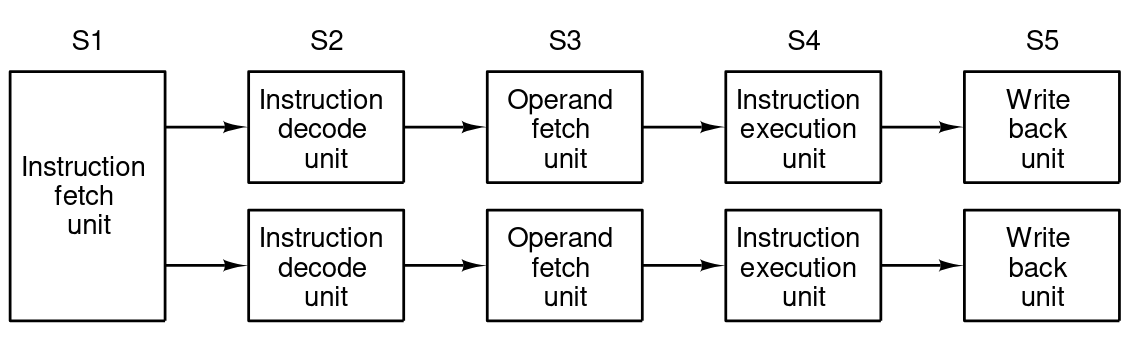
\includegraphics[scale=0.2]{2pip}
\end{center}

\paragraph{Specialized execution units}
\begin{center}
	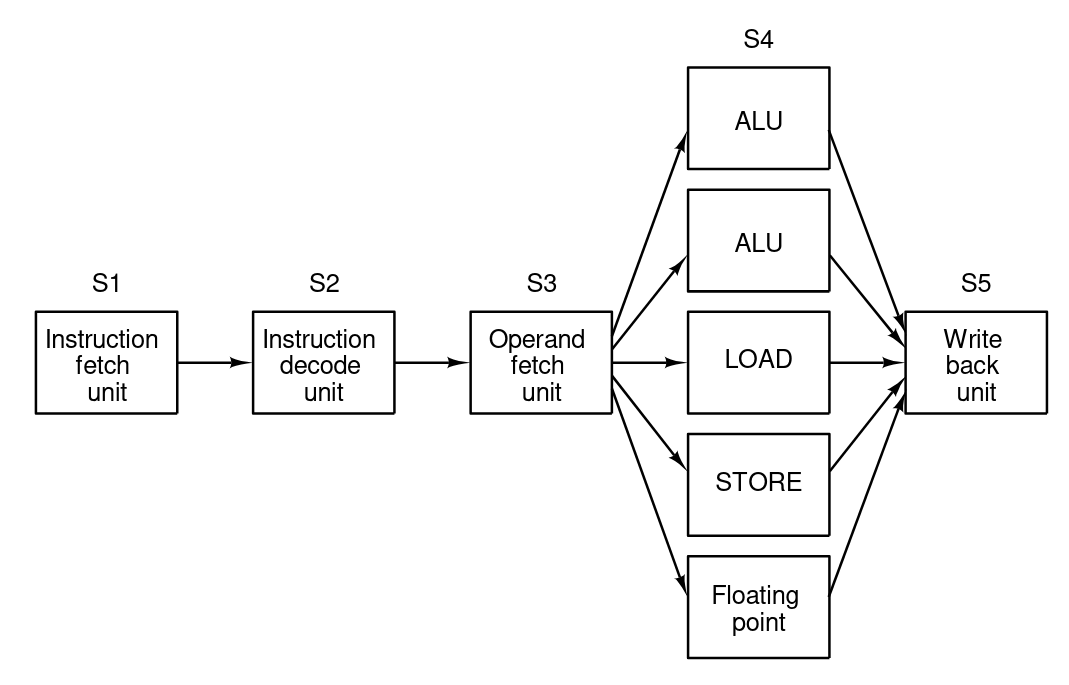
\includegraphics[scale=0.3]{specexe}
\end{center}

\paragraph{MIPS pipeline}
The MIPS pipeline is defined as follows:
\begin{enumerate}
	\item \textbf{Instruction Fetch} (IF): fetch instruction from \textit{main} memory
	\item \textbf{Instruction Decode} (ID): read operand registers while decoding the instruction (simultaneous thanks to format of MIPS instructions)
	\item \textbf{Execution} (EXE): \textbf{execute} the operation (arithmetical and logical operations) or \textbf{calculate} an address (\textit{load} and \textit{store})
	\item \textbf{Memory Access} (MEM): access an operand in data memory\footnote{If the instruction is \textit{load} or \textit{store}, otherwise nothing happens.}
	\item \textbf{Write Back} (WB): write the result into a register
\end{enumerate}
With this pipeline the affected registers are \textbf{written} into during the first half of the WB stage while the operand registers are \textbf{read} during the second half of the ID stage.

\begin{center}
	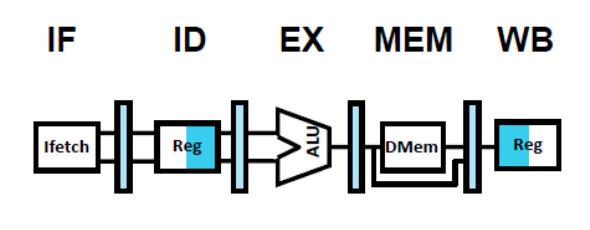
\includegraphics[scale=0.4]{mips}
\end{center}

\subsubsection{Pipeline hazards}
\begin{definition}[Pipeline hazard]
	Phenomena that may disrupt the smooth execution of a pipeline.
\end{definition}

\begin{example}
	If we assume a unified cache with a single read port (instead of separate instruction and data caches), a memory read conflict appears among IF and OF stages. The pipeline has to stall (\textbf{pipeline bubble}) one of the accesses until the required memory port is available.
\end{example}

\hfill

\paragraph{Data hazard} These type of hazards happen when there are \textbf{dependencies} between instructions, causing an overlapping between their execution. There are three types:
\begin{itemize}
	\item \textbf{Read After Write} (RAW): instruction 2 tries to read the register before instruction 1 writes it
	\item \textbf{Write After Read} (WAR): instruction 2 tries to write a register before instruction 1 reads it
	\item \textbf{Write After Write} (WAW): instruction 2 writes a register before instruction 1 writes it
\end{itemize}

\begin{example}[RAW in MIPE pipeline]
	Let's consider this piece of code:
	\begin{lstlisting}[language={[x86masm]Assembler}]
		mov R1, A
		mov R2, B
		add R2, R1, R2
		mul R1, R2, R1
	\end{lstlisting}
	We will have the following dependencies:
	\begin{center}
		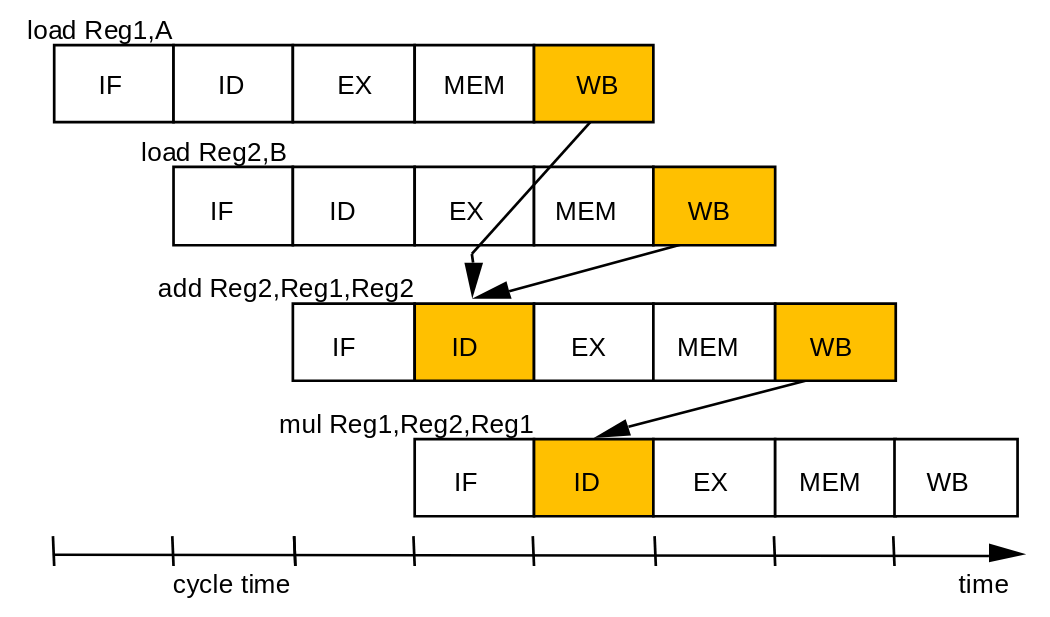
\includegraphics[scale=0.3]{rawex}
	\end{center}
\end{example}

\begin{observation}[WAR and WAW]
	In a five stage pipeline WAR and WAW can't happen since all instructions take five stages and the reads are always in stage 2 while the writes in stage 5.
\end{observation}

\subparagraph{Software solutions}
Software solutions involve two options:
\begin{itemize}[leftmargin=+1.5cm]
	\item Put \textbf{no-op} operations after each instruction that may cause a hazard
	\item \textbf{Reorder} the instructions
\end{itemize}

\subparagraph{Hardware solutions}
Hardware solutions require a hazard detection logic:
\begin{itemize}[leftmargin=+1.5cm]
	\item \textbf{Stalling} or \textbf{interlocking}: we stall the pipeline for one or more cycles
	\item \textbf{Forwarding}: we forward either the \textbf{result} or the \textbf{load}ed data directly to the next stage where it's needed. It may be necessary to also use \textbf{stalling} since even if forwarded the data may still not be available.
\end{itemize}

\newpage
\begin{example}[Forwarding]
	Let's consider this piece of code:
	\begin{lstlisting}[language={[x86masm]Assembler}]
		add R1, R2, R3
		sub R4, R1, R3
		and R6, R1, R7
		or R8, R1, R9
	\end{lstlisting}
	We will have the following forwarding of both, result and load
	\begin{center}
		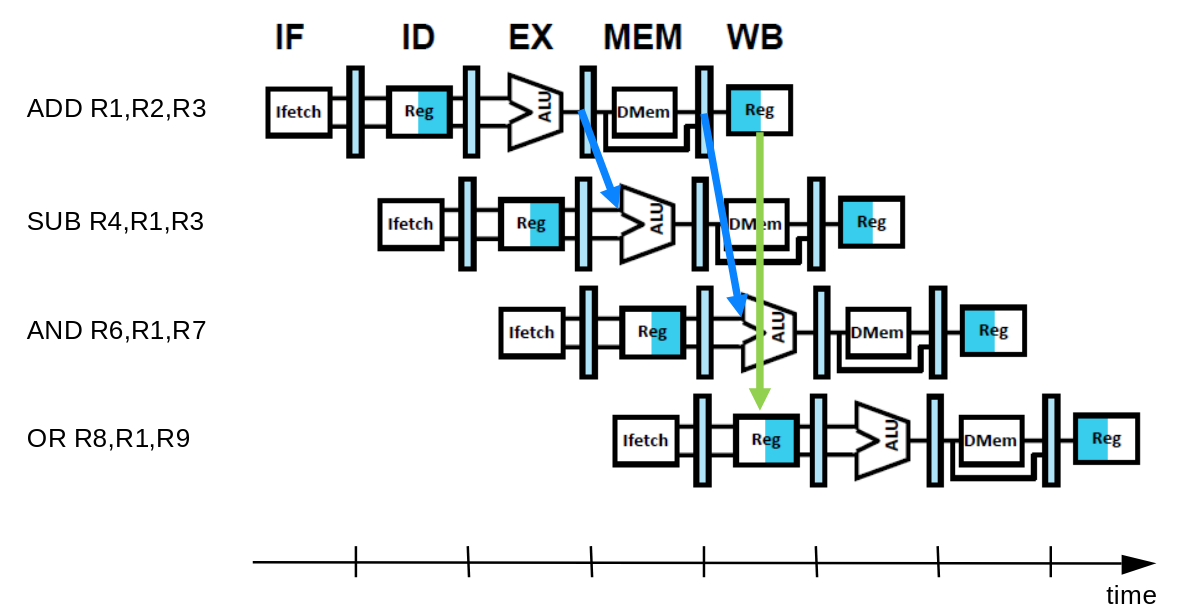
\includegraphics[scale=0.3]{fwex}
	\end{center}
\end{example}

This is how a hardware (\textbf{bypass}) solution can be implemented:
\begin{center}
	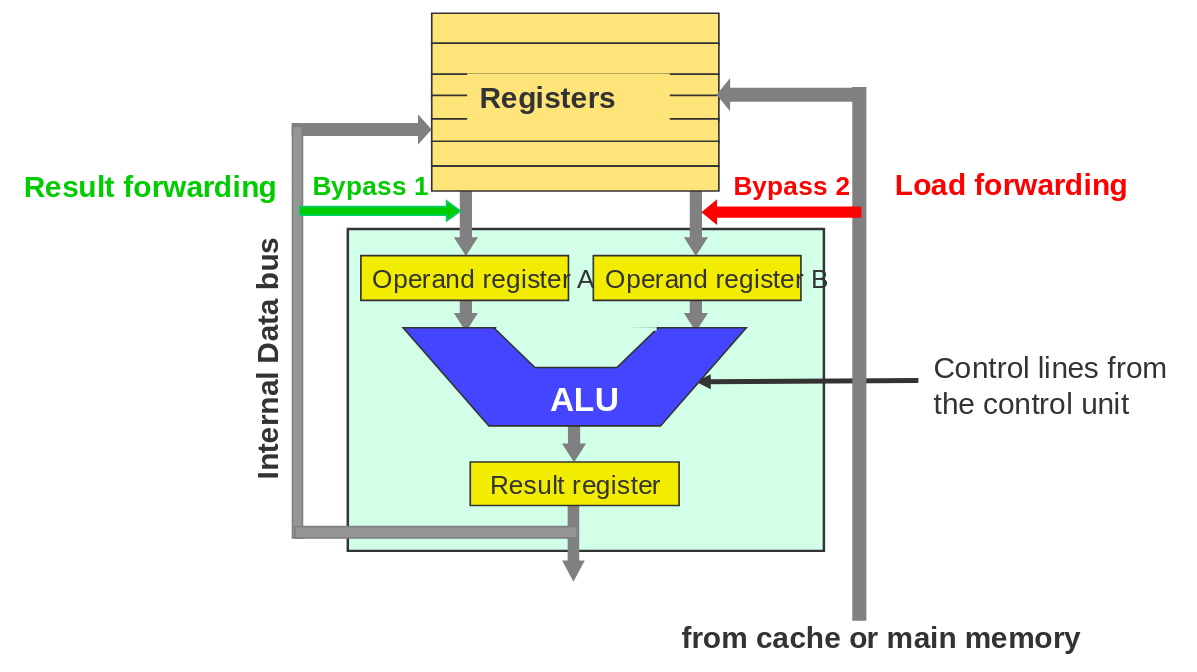
\includegraphics[scale=0.4]{byp}
\end{center}
\newpage

\paragraph{Structural hazard}
Structural hazards may arise from some combinations of instructions that cannot be accommodated because of \textbf{resource conflicts}.
\begin{example}
	If the processor has only one register port and two instructions want to write into it at the same time.
\end{example}

The main solutions are:
\begin{itemize}
	\item \textbf{Arbitration with interlocking}: hardware that performs resource conflict arbitration and interlocks one of the competing instructions
	\item \textbf{Resource replication}: e.g. more write ports. This could arise more dependencies.
\end{itemize}

\paragraph{Control hazard}
Control hazards arise from \textbf{control flow instructions} (e.g. branch, jump).
\begin{example}
	Considering this code:
	\begin{lstlisting}[language={[x86masm]Assembler}]
						cmp R1,R2
						adc R4,R5,R4
						beq Label
						add R3,R1,R2
		Label: 		sub R6,R4,R5
						sll R0
	\end{lstlisting}
	The \textit{add} instruction is still in the pipeline when the jump is executed and therefore it is also executed before it.
	
	\subparagraph{Software solution}
	There are two options:
	\begin{itemize}[leftmargin=+1.5cm]
		\item Put \textbf{no-op} operations after every branch
		\item \textbf{Reorder} the instructions so that the ones that will not affect the branch will be executed right before it
	\end{itemize}
	\subparagraph{Hardware solution}
	There are three options:
	\begin{itemize}[leftmargin=+1.5cm]
		\item \textbf{Interlocking}: the hardware detects the branch and applies the interlocking to stall the next instructions
		\item \textbf{Flushing}: empty the pipeline before releasing the jump
		\item \textbf{Speculative branch}: in case of a \textbf{conditional jump} estimate the result and load the pipeline. If the estimate was wrong, \textit{flush}.
	\end{itemize}
\end{example}

\subsubsection{Branch prediction}
Branch prediction foretells the outcome of conditional branch instructions. IF stage finds a branch instruction and predicts its direction. The branch delay slots are speculatively filled with instruction, either those of:
\begin{itemize}
	\item the consecutively \textbf{following path},
	\item the path at the \textbf{target address}
\end{itemize}
After resolving of the branch direction decide upon correctness of prediction. In case of misprediction discard wrongly fetched instructions. Re-rolling in this case is \textbf{expensive}.

\paragraph{Branch Target Buffer}
The Branch Target Buffer (BTB) or Branch-Target Address Cache (BTAC) stores branch and jump target
addresses. The BTB is accessed during the IF stage and consists of a table with \textbf{branch addresses}, the corresponding \textbf{target addresses}, and \textbf{prediction information}.
There are some variations:
\begin{itemize}
	\item \textbf{Branch Target Cache} (BTC): stores one or more target instructions additionally
	\item \textbf{Return Address Stack} (RAS): a small stack of return addresses for procedure calls and returns is used additional to and independent of a BTB.
\end{itemize}

\paragraph{Static}
The prediction for an individual branch	does not change and comprises of:
\begin{itemize}
	\item \textbf{machine-fixed}: the prediction can be \textbf{wired} into the processor by predicting that all branches will be taken (backwards) or all not taken (forward)
	\item \textbf{compiler-based}: opcode in branch instructions allows the compiler to set it. Then it can either \textbf{examine} the program code or use \textbf{profile information} from earlier runs
\end{itemize}
\paragraph{Dynamic}
In dynamic branch prediction the prediction is decided on the \textbf{computation history} of the program execution. In general gives better results than static but at the cost of \textbf{increased hardware complexity}.
\subparagraph{Predictors}
A \textbf{one-bit} predictor correctly predicts a branch at the end of a loop iteration, as long as the loop does not exit. In nested loops, a one-bit prediction scheme will cause two mispredictions for the inner loop:
\begin{itemize}
	\item One at the \textbf{end} of the loop, when the iteration exits the loop instead of looping again
	\item One when executing the \textbf{first loop iteration}, when it predicts exit instead of looping
\end{itemize}
This is avoided by a \textbf{two-bit} predictor scheme, where a prediction must miss twice before it is changed when a two-bit prediction scheme is applied.
\begin{figure}[!h]
	\centering
	\subfigure[one-bit]{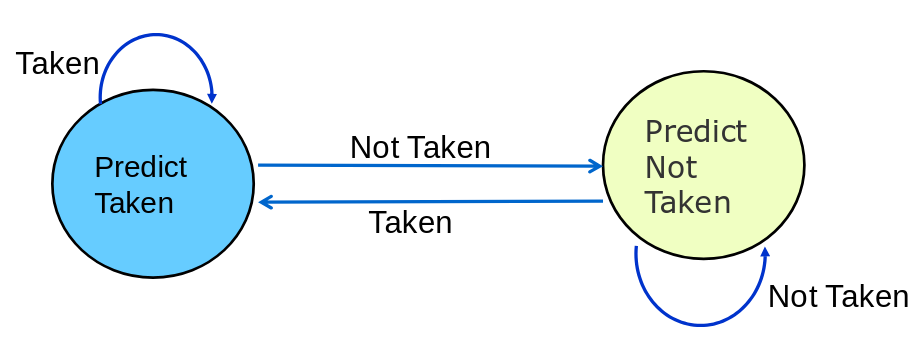
\includegraphics[scale=0.23]{onebit}}
	\hfill\\
	\subfigure[two-bit Hysteresis scheme]{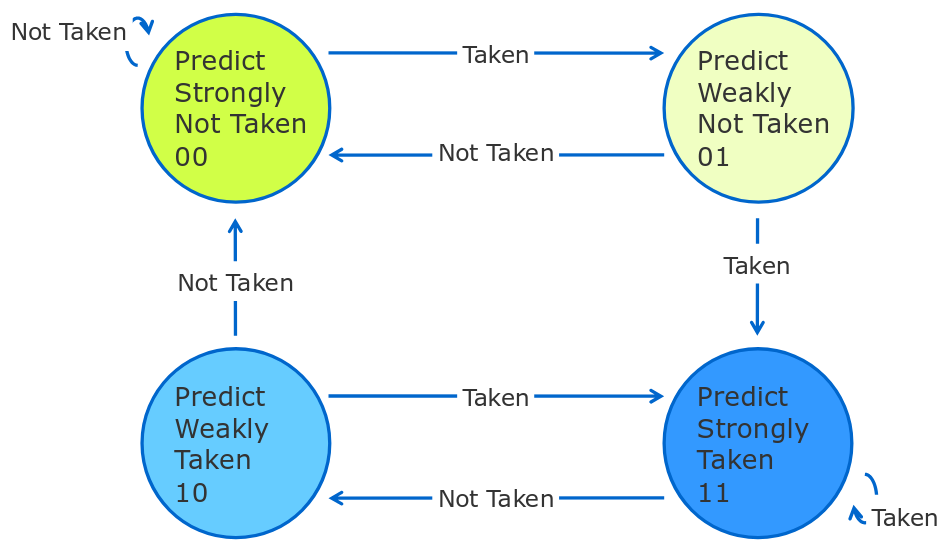
\includegraphics[scale=0.23]{twobit}}
	\hfill
	\subfigure[two-bit 	Saturation Counter scheme]{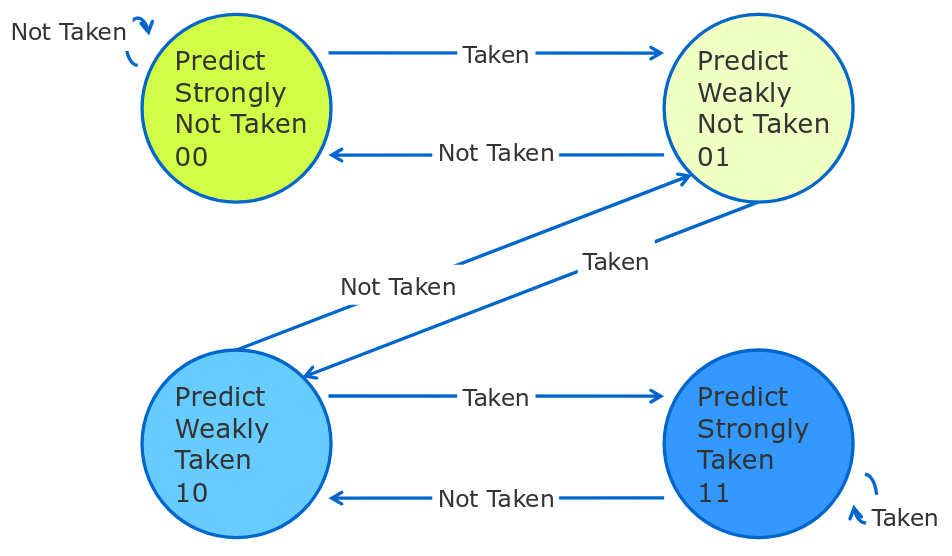
\includegraphics[scale=0.23]{twobitsat}}
	\hfill
\end{figure}

\begin{center}
	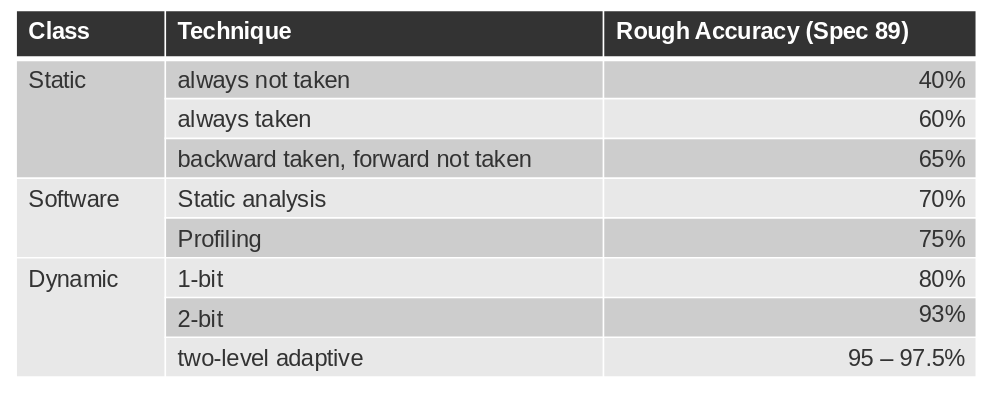
\includegraphics[scale=0.3]{predstat}
	\captionof{figure}{Statistics about different techniques}
\end{center}

\paragraph{Predicate instructions}
It provides \textbf{predicated} or \textbf{conditional instructions} and \textbf{predicate registers}, which are used as an additional input operand. They are able to remove a branch and keep the pipeline busy but it complicates the instruction set and consume resources.

\subsection{Superscalar processors}
\begin{definition}
	Superscalar machines are distinguished by their ability to dynamically issue multiple instructions each clock cycle from a conventional linear instruction stream.
\end{definition}

\begin{center}
	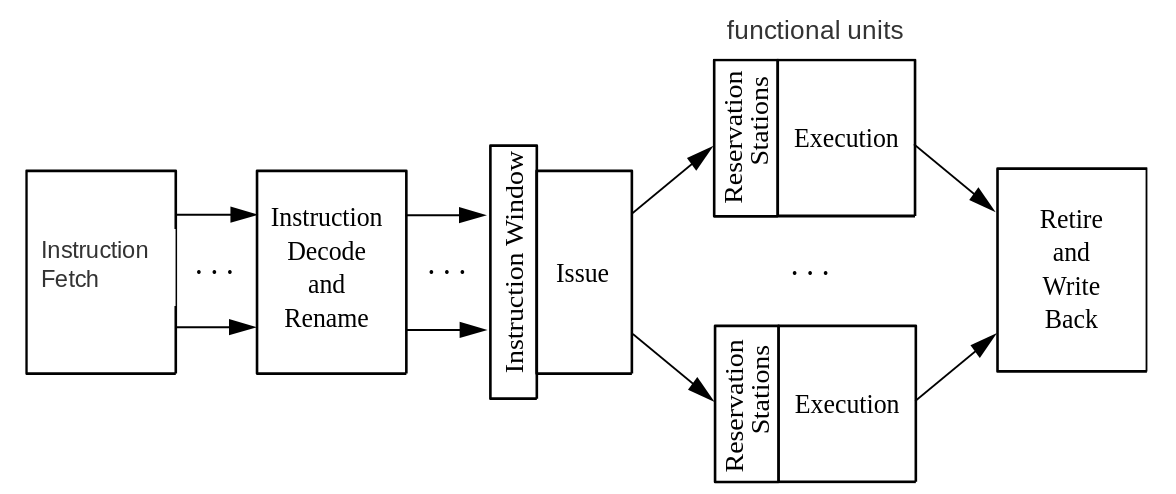
\includegraphics[scale=0.35]{super}
\end{center}

A superscalar pipeline is divided in three sections:
\begin{itemize}
	\item \textbf{in-order}
	\begin{itemize}
		\item \textit{fetch}: get the commands
		\item \textit{decode}: decode the new instructions
		\item \textit{rename}: externally visible register are mapped to internal shadow registers, stored in a rename map (e.g. \textit{alias table}), so that core execution units are free from name dependencies
		\item \textit{issue} if \textit{in-order} issue processor. The waiting instructions in the \textbf{waiting window} are examined and then simultaneously (up to the \textit{issue bandwidth}) \textbf{issued} to the \textbf{functional units}
	\end{itemize}
	\item \textbf{out-of-order}
	\begin{itemize}
		\item \textit{issue} if out-of-order issue processor
		\item \textit{execution}: there is a \textbf{reservation station}, a buffer that contains a single instruction operands. There may be one for multiple units. When all the operands are ready the instruction is \textbf{dispatched}.
		\item \textit{completion}: when the result is ready for forwarding and buffering. The reservation station gets freed and the state of the execution (can be an interrupt) is noted in the \textbf{reorder buffer}
		\item \textit{Commitment}: after completion an instruction gets committed if:
		\begin{itemize}
			\item al previous instructions are committed or can be committed in the same cycle
			\item if no interrupt occurred before and during the execution
			\item if the instruction is not speculative anymore
		\end{itemize}
	\end{itemize}
	\item \textbf{in-order}
	\begin{itemize}
		\item \textit{retirement}: an instruction retires when the reorder buffer is freed either because of a commit or a delete
		\item \textit{write-back}: the result of the instruction is made permanent in the architectural register
	\end{itemize}
\end{itemize}